\section{Forward Security}
\label{sec:forward-sec}

\paragraph{Motivation} Until now, we have used a secret key that was only known by one or more honest parties participating in the various protocols.
However in the real world, the secret key often gets compromised, and the adversary learns some information about it.
This might happen if the device gets stolen or confiscated, if the honest parties get hacked or just through human error.
If we use our KEM from Figure~\ref{fig:kem:const:elgamal} as an example, this would enable the adversary to decapsulate every single ciphertext that was sent (if the adversary recorded the ciphertexts).
Forward Security guarantees that messages before the compromise remain secure (Figure~\ref{fig:fs:sketch}).

In this section, we will discuss how to achieve security even if the secret key is compromised in the future, using our KEM as an example.

\begin{figure}[!ht]
    \centering
    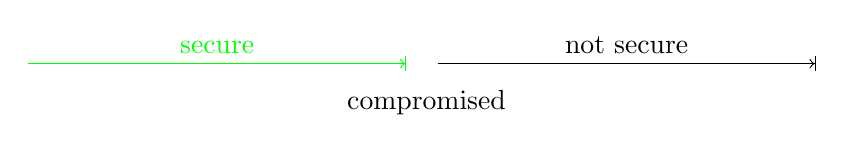
\begin{tikzpicture}%
    \draw [green, -{>Bar}] (0,0) -- (4.8,0) node [midway, above] {secure};
    \node at (5,0) {\LARGE\Lightning};
    \node at (5,-.5) {$\dk$ compromised};
    \draw [-{>Bar}] (5.2,0) -- (10,0) node [midway, above] {not secure};
\end{tikzpicture}%
    \caption{A sketch of forward security}
    \label{fig:fs:sketch}
\end{figure}

\subsection{Forward Secure KEMs}

\paragraph{Syntax} To provide security even if the secret key is leaked, we have to change the secret key over time.
This means we also need to change the syntax of the decapsulation algorithm.
The forward-secure KEM $\FKEM=(\FKEMgen,\FKEMenc,\FKEMdec)$ is a tuple of three algorithms with encapsulation key space~$\eksp$, decapsulation key space~$\dksp$, ciphertext space~$\csp$, and symmetric key space~$\ksp$:
\begin{itemize}
    \item $\KEMgen: \emptyset \tor \dksp\times\eksp$
    \item $\KEMenc: \eksp \tor \ksp\times\csp$
    \item $\KEMdec: \dksp\times\csp \to \dksp\times\ksp$
\end{itemize}

\paragraph{Correctness} A forward-secure KEM $\FKEM$ is correct if $\Pr[\CORR_{\FKEM}(\advA)=0]=1$ for all adversaries~$\advA$, where game~$\CORR$ is defined in Figure~\ref{fig:fkem:corr}.

\begin{figure}[!ht]
    \centering
    \nicoresetlinenr%
    \fbox{%
        \scalebox{\codescalefactor}{%
            % !TeX root = ..\..\main.tex
\markersetlen{ndL}{120pt}%
\markersetlen{ndR}{130pt}%
\newcommand{\CK}{\mathit{CK}}%
\begin{tabular}[t]{ll}
    \nicodemusbox{\markerlenndL}{%
        \textbf{Game} $\CORR_{\FKEM}(\advA)$
        \begin{nicodemus}
            \item $\CK[\cdot]\gets\bot$
            \item $(\dk,\ek)\getsr\FKEMgen$
            \item Invoke $\advA(\ek)$
            \item Stop with~$0$
        \end{nicodemus}%
        \medskip
        
        \textbf{Oracle} $\Oenc$
        \begin{nicodemus}
            \item $(k,c)\getsr\FKEMenc(\ek)$
            \item If $\CK[c]\neq\diamond$: $\CK[c]\gets k$
            \item Return~$c$
        \end{nicodemus}%
    }%
    &
    \nicodemusbox{\markerlenndR}{%
        \textbf{Oracle} $\Odec(c)$
        \begin{nicodemus}
            \item $(\dk,k')\gets\FKEMdec(\dk,c)$
            \item If $\CK[c]\notin\{k',\bot,\diamond\}$:
            \item \quad Stop with $1$
            \item If $\CK[c]\neq\bot$: $\CK[c]\gets \diamond$
            \item Return $k'$
        \end{nicodemus}%
    }%
\end{tabular}%%
        }%
    }
    \caption{%
        Game $\CORR$ for forward-secure KEM~$\FKEM$.
    }
    \label{fig:fkem:corr}
\end{figure}



\paragraph{Security}
The advantage of an adversary~$\advA$ against forward-secure KEM $\FKEM$ in game $\INDCCA$ from Figure~\ref{fig:fkem:ind} is defined as:
\[
\Adv_\FKEM^\indcca(\advA)\coloneqq\left|\Pr[\INDCCA_{\FKEM}^0(\advA)=1]-\Pr[\INDCCA_{\FKEM}^1(\advA)=1]\right|\text{.}
\]

\begin{figure}[!ht]
    \centering
    \nicoresetlinenr%
    \fbox{%
        \scalebox{\codescalefactor}{%
            % !TeX root = ..\..\main.tex
\markersetlen{ndL}{130pt}%
\markersetlen{ndR}{130pt}%
\newcommand{\CC}{\mathit{CC}}%
\begin{tabular}[t]{ll}
    \nicodemusbox{\markerlenndL}{%
        \textbf{Game} $\INDCCA_{\FKEM}^b(\advA)$
        \begin{nicodemus}
            \item $x\gets 0$
            \item $\CC\gets\emptyset$
            \item $(\dk,\ek)\getsr\FKEMgen$
            \item $b'\getsr\advA(\ek)$
            \item Stop with~$b'$
        \end{nicodemus}%
        \medskip
        
        \textbf{Oracle} $\Ochall$
        \begin{nicodemus}
            \item If $x=1$: Return $\bot$
            \item $(k_0,c)\getsr\FKEMenc(\ek)$
            \item $k_1\getsr\ksp$
            \item $\CC\gets\CC\cup\{c\}$
            \item Return~$(k_b,c)$
        \end{nicodemus}%
    }%
    &
    \nicodemusbox{\markerlenndR}{%
        \textbf{Oracle} $\Odec(c)$
        \begin{nicodemus}
            \item $(\dk,k)\gets\FKEMdec(\dk,c)$
            \item If $c\in\CC$: $k\gets\bot$
            \item $\CC\gets\CC\setminus\{c\}$
            \item Return $k$
        \end{nicodemus}%
        \medskip
        
        \textbf{Oracle} $\Ocorrupt$
        \begin{nicodemus}
            \item Require $\CC=\emptyset$
            \item Return~$\dk$
        \end{nicodemus}%
    }%
\end{tabular}%%
        }%
    }
    \caption{%
        Games $\INDCCA$ for forward-secure KEM~$\FKEM$.
    }
    \label{fig:fkem:ind}
\end{figure}

\paragraph{Trivial winning strategies} In addition to the trivial winning strategies for Game~$\INDCCA^b_\KEM$ from Section~\ref{sec:kem:trivial_attacks}, two new trivial attacks have to be considered (Figure~\ref{fig:fkem:triv}).

\begin{figure}[!ht]%
    \centering
    %!TEX root=../main.tex
\parbox[t]{5cm}{%
    \begin{enumerate}[topsep=0pt]
        \item $\Ocorrupt\to\dk$
        \item $\Ochall\to(k,c)$
        \item $(\dk',k')\gets\FKEMdec(\dk,c)$
    \end{enumerate}
}\parbox[t]{5cm}{%
    \begin{enumerate}[topsep=0pt]
        \item $\Ochall\to(k,c)$
        \item $\Ocorrupt\to\dk$
        \item $(\dk',k')\gets\FKEMdec(\dk,c)$
    \end{enumerate}
}
    \caption{Additional Trivial winning strategies for forward-secure KEMs.}
    \label{fig:fkem:triv}
\end{figure}
